\section{Performance Evaluation}
The extension's performance goals are to provide our security guarantees without being a detriment to the end user's browsing experience. All of our timestamps were recorded using the Performance Web API. While our extension's functionality only applies at the network level, there is potential slowdown at the DOM processing level. Figure ~\ref{fig:navigationtiming} presents shows the different timestamps provided by the Navigation Timing API, as well as a high-level description of the browser processing model. Since our filter listens on the onBeforeRequest event, none of the previous steps before Request are affected. In this section, we refer to the difference in time between responseEnd and requestStart as the "network filter time".

\begin{figure}[h]
 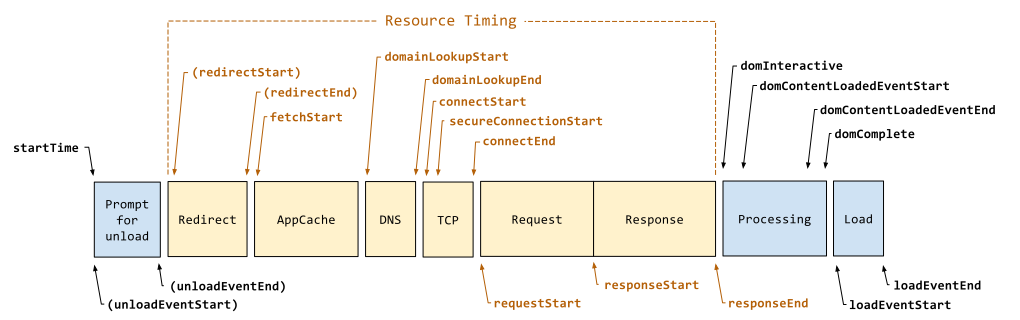
\includegraphics[scale=0.32]{img/timestamp-diagram}
 \caption{The Navigation Timing API's timestamps}
 \label{fig:navigationtiming}
 \end{figure}

\subsection{Top websites load times}
We first report our extension's impact on top website load times, representing the expected behaviour of an user's average web browsing experience. For these tests, we first took the top 500 websites as reported by Moz.com \cite{top500}. For each website, we loaded it 20 times (with a 25 second timeout) and recorded the following values: requestStart, responseStart, responseEnd, domContentLoadedEventEnd, domComplete, duration, and decodedBodySize. From the initial 500, we only report values for 441 of them. The other 59 had consistent issues with timeouts, insecure certificates, and network errors. For our setup, we used a headless version of Firefox, and Selenium WebDriver for NodeJS, with GeckoDriver. We ran four test suites:
\begin{itemize}
	\item No extension cold cache: Firefox is loaded without the extension installed and the web driver is re-instantiated for every page load.
	\item Extension cold cache: Firefox is loaded with the extension installed and the web driver is re-instantiated for every page load.
	\item No extension warm cache: Firefox is loaded without the extension installed and the same web driver is used for the page's 20 loads.
	\item Extension warm cache: Firefox is loaded with the extension installed and the same web driver is used for the page's 20 loads.
\end{itemize}

The recorded timestamps do not hold much value by themselves, only when analysed with regards to each other. Thus, for each set of tests, we reduced the recorded values to three comparisons: responseStart (responseStart - requestStart), responseEnd (responseEnd - requestStart), and domResponse (domComplete - responseStart). The first two analyze the time spent by the network filter, while the third determines the time spent until the whole document has loaded. We calculate the medians of each website for each of the previous three values and the decodedByteSize.

\begin{figure}[h]
	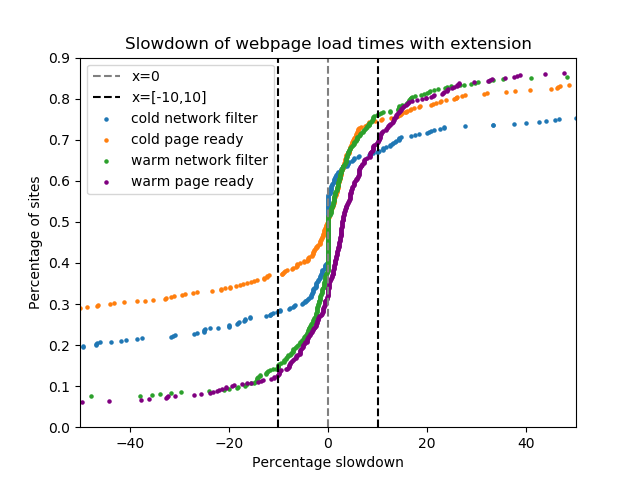
\includegraphics[scale=0.5]{results/extension_slowdown_overall}
	\caption{Cumulative distribution of relative percentage slowdown with extension installed for top sites}
	\label{fig:overall_slowdown}
\end{figure}

We compare the load times with and without the extension running by calculating the relative slowdown with the extension installed. Figure ~\ref{fig:overall_slowdown} shows the computed results. The graph shows that the slowdown is not too great when the extension is running. Note that these values are recorded as percentages, and while some are as high as 50\%, the absolute values are in the order of seconds, and in many cases tens or hundreds of milliseconds, especially for the network component. Such values should not alter the user's experience significantly. The slowdown increases when we take caching into account. We expect this to be the case because the network filter probably causes the browser to use less caching, especially for the DOM component, as it might have to process it from scratch every time.

\begin{figure}[h]
	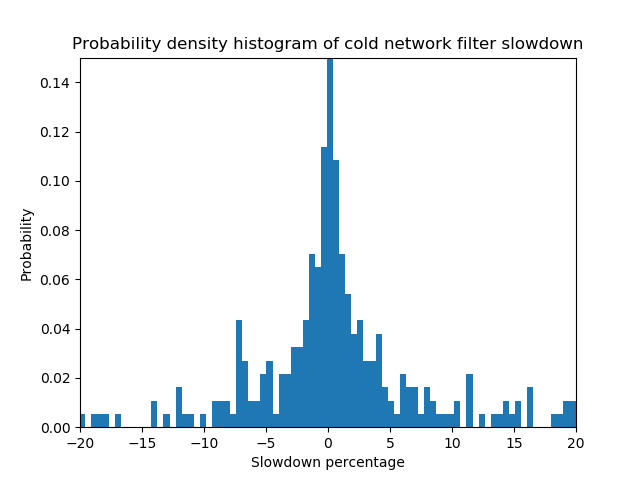
\includegraphics[scale=0.5]{results/density_histogram_filter_slowdown}
	\caption{Density histogram of network filter slowdown for top sites}
	\label{fig:histogram_slowdown}
\end{figure}


Figure ~\ref{fig:histogram_slowdown} shows a closer look at the distribution for the network filter slowdown on the top sites. We see that for this component, most of the slowdown is centred around [-10\%,10\%].

\begin{figure}[h]
	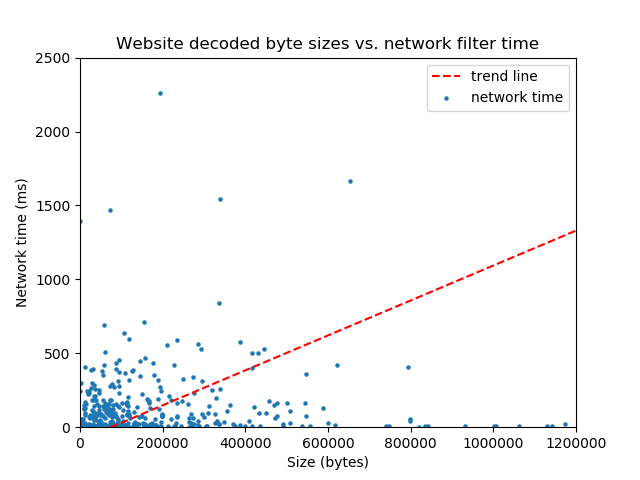
\includegraphics[scale=0.5]{results/byte_size_vs_filter_time}
	\caption{Scatter plot of network filter time as a function of decoded byte size for top sites}
	\label{fig:network_filter_decoded_size}
\end{figure}

\begin{figure}[h]
	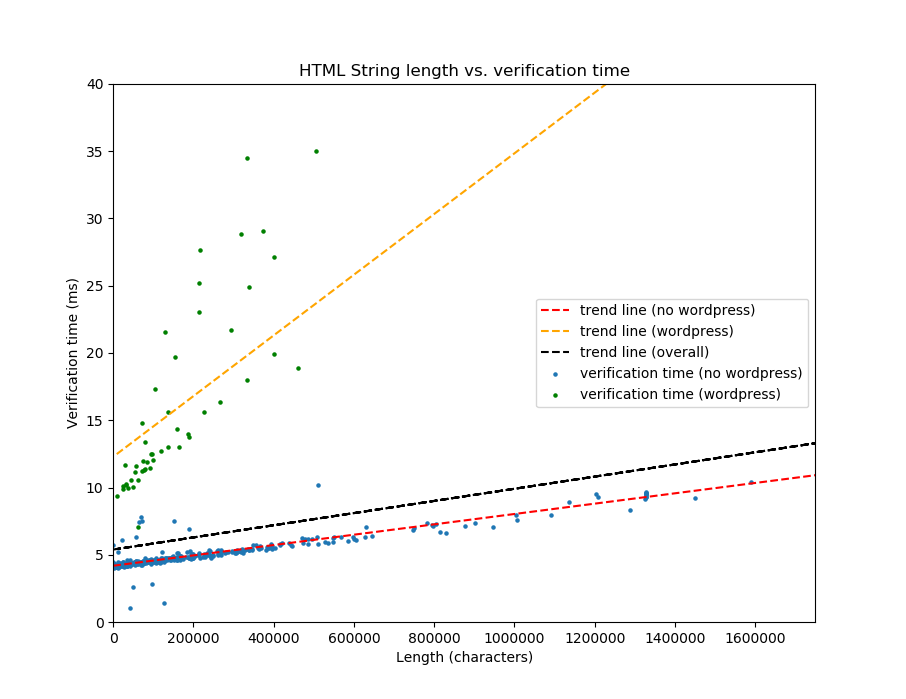
\includegraphics[scale=0.4]{results/string_length_vs_verification_time}
	\caption{Scatter plot of network filter time as a function of decoded byte size for top sites}
	\label{fig:verification_time_string_length}
\end{figure}

Figure ~\ref{fig:network_filter_decoded_size} shows the network filter time as a function of the page's decoded byte size. Applying least squares regression shows an upwards trend. However, the Spearman's rank correlation for this set of data is 0.02 (TODO: change this value when new data comes in); we believe this to be due to the number of factors affecting this measurement. In order to obtain a more accurate quantification of this data, we measured the time spent by the call to the HTML string verification function in our network filter, and the length of the string to be verified. As before, we loaded the same websites 20 times each and calculated the median times and lengths. Figure ~\ref{fig:verification_time_string_length} shows the results. The blue dots are the pages for which the WordPress probes tested negative, and the green dots are the pages for which the probes tested positive: 55 in total (our implementation currently only has probes for WordPress). As in the previous graph, we applied least squares regression to calculate the shown trend lines. The Spearman's rank correlation values for no WordPress, WordPress, and overall are 0.78, 0.91, and 0.60 respectively, demonstrating positive correlation. Since both our probes and signatures use regex matching, we expect both trend lines to be linear, as seen in the graph. Recall that once a probe for a certain software passes, we do a linear scan over the signatures for that specific software and check whether it applies to the given HTML string or not. Thus, we expect the slope of the line to be higher when the WordPress probe passes. Since only around 25\% of sites use WordPress on average \cite{w3techs}, we expect the impact of our network filter to be closer to the non-WordPress values, as corroborated by our overall trend line.

Additionally, for each website we recorded the number of loaded signatures (i.e. signatures whose endpoints were found in the HTML). None of the websites loaded any signatures, even though some of the sites tested positive for WordPress. Thus, we can infer with confidence that the rate of false positives for loaded signatures during an average user's web browsing is extremely low. While we can not be sure that any of the sites is free of vulnerabilities described in our current signatures, this is very unlikely, as many of these websites are not running WordPress to begin with, and being some of the most popular, they would likely be updated relatively quickly if any vulnerability is found; thus, the rate of false negatives is likely extremely low as well. It is reasonable to assume that the rate of false positives for loaded signatures would go up for a WordPress site. Since most of the tested sites are not running WordPress, this might have skewed the probability down. TODO: can we calculate a conclusive value for false positives of loaded signatures out of the number of websites running wordpress?)



